\section{Empirical Validation}
\label{sec:empirical_validation}

To overcome the ``Validation Gap'' documented by Wendler~\cite{wendler_2012} and fulfill Requirement \textbf{R3} of Becker et al.\~\cite{becker_2009}, we evaluate the CN-OMM using a multi-methodological strategy aligned with Helgesson et al.'s evaluation taxonomy~\cite{helgesson_2012}: (i) a \textbf{Type-1 Methodological \& Structural Audit} verifying compliance with DSR requirements R1--R8, and (ii) a \textbf{Type-3 Real-System Controlled Empirical Experiment} on a production-grade Kubernetes microservice benchmark subjected to Chaos Engineering fault injection.

\subsection{Type-1 Evaluation: DSR Compliance Audit (Becker R1--R8)}
\label{subsec:type1_evaluation}

Table~\ref{tab:becker_evaluation} summarizes the verification of the CN-OMM against Becker, Knackstedt, and P\"{o}ppelbu\ss's eight mandatory DSR requirements~\cite{becker_2009}. Unlike conceptual models that rely on ad-hoc stage labels~\cite{patel_2025, grafana_omm_2024}, CN-OMM satisfies every methodological criterion: it is grounded in a systematic comparison against seven prior frameworks (R1), evolved iteratively across literature synthesis, mathematical modeling, and chaos calibration (R2), combines theoretical and empirical validation (R3, R4), addresses well-defined cloud-native diagnostic and FinOps bottlenecks (R5, R6), and delivers both practitioner-ready matrices and reproducible open-source audit scripts (R7, R8).

\begin{table*}[t]
\centering
\caption{Methodological Alignment of the CN-OMM with Becker et al.'s Eight DSR Requirements (R1--R8) and Helgesson et al.'s Evaluation Taxonomy}
\label{tab:becker_evaluation}
\footnotesize
\setlength{\tabcolsep}{4.5pt}
\renewcommand{\arraystretch}{1.18}
\begin{tabularx}{\textwidth}{l l >{\raggedright\arraybackslash}X l}
\toprule
\textbf{Code} & \textbf{DSR Requirement~\cite{becker_2009}} & \textbf{Instantiation and Methodological Implementation in the CN-OMM Artifact} & \textbf{Section / Evidence} \\
\midrule
\textbf{R1} & Comparison with existing models & Systematic audit of 7 existing academic and industrial frameworks (~\cite{duarte_2013, patel_2025, amgothu_2025, grafana_omm_2024, dynatrace_omm_2024, cncf_obs_2024, wwt_omm_2025}), proving the need for formal cross-pillar and probe-effect dimensions. & Section~\ref{sec:critical_analysis}, Table~\ref{tab:existing_models_comparison} \\
\textbf{R2} & Iterative procedure & Three-iteration design cycle: (i) Rapid Review taxonomy synthesis; (ii) mathematical state-space \& configurational refinement; (iii) empirical chaos calibration. & Sections~\ref{sec:background}--\ref{sec:empirical_validation} \\
\textbf{R3} & Evaluation & Dual evaluation following Helgesson et al.\~\cite{helgesson_2012}: Type-1 structural/theoretical grounding and Type-3 controlled Kubernetes chaos experiments ($N=30$ \& $N=60$). & Section~\ref{sec:empirical_validation}, Table~\ref{tab:empirical_validation} \\
\textbf{R4} & Multi-methodological procedure & Combines Literature Synthesis, Control-Theoretic State Formalization, Declarative Automated Auditing (Proen\c{c}a~\cite{proenca_2016_rcis}), and Factorial Chaos Experimentation. & Sections~\ref{sec:cn_omm}--\ref{sec:empirical_validation} \\
\textbf{R5} & Identification of problem relevance & Addresses the diagnostic collapse of monomodal tracing and uncontrolled telemetry FinOps/CPU overhead in production Kubernetes microservices. & Section~\ref{sec:introduction} \\
\textbf{R6} & Problem definition & Defines the domain scope (cloud-native Kubernetes clusters), target users (SREs, platform architects), and non-compensatory stage-gate constraints. & Sections~\ref{sec:introduction}, \ref{sec:cn_omm} \\
\textbf{R7} & Targeted presentation of results & Provides both a $5\times5$ architectural matrix for practitioners and a declarative Python/PromQL automated assessment engine (\texttt{evaluate\_cn\_omm.py}). & Tables~\ref{tab:cn_omm_dimensions}--\ref{tab:cn_omm_matrix}, Section~\ref{sec:assessment} \\
\textbf{R8} & Scientific documentation & Full Open Science replication package including formal equations, cluster audit datasets, raw chaos trial logs, and statistical reproduction scripts. & Section~\ref{sec:conclusion} \\
\bottomrule
\end{tabularx}
\end{table*}


\subsection{Type-3 Evaluation: Experimental Design and Kubernetes Testbed}
\label{subsec:type3_design}

To address Research Question \textbf{RQ3}, we instantiated three operational observability architectures corresponding to CN-OMM Levels 2, 3, and 4 on a multi-node Kubernetes cluster (v1.30, containerd runtime, Linux kernel 6.6) hosting the polyglot \textbf{CNCF OpenTelemetry Astronomy Shop} microservice benchmark~\cite{opentelemetry_demo, wang2024building} (14 interconnected services in Go, Rust, Python, Java, TypeScript, .NET, and C++ under continuous Locust~\cite{locust_framework} load generation):
\begin{enumerate}[leftmargin=*, nosep]
    \item \textbf{Baseline A -- Native CLI Regime (CN-OMM Level 2):} Relies on standard Kubernetes control-plane events, \texttt{kubelet}/cAdvisor metrics, and automated CLI diagnostic scraping (\texttt{kubectl get/describe pods}, \texttt{kubectl top}, \texttt{kubectl logs}) without distributed context propagation.
    \item \textbf{Baseline B -- Monomodal Tracing Regime (CN-OMM Level 3 Attempt):} Deploys OpenTelemetry SDKs exporting distributed traces to Jaeger/Tempo, ranking root-cause candidates by maximum inclusive span tail latency $P_{95}(D(s_i))$ without cross-pillar log/metric correlation or exclusive self-time isolation ($D_2 = 2.3$).
    \item \textbf{Treatment -- Correlated Multimodal Regime (CN-OMM Level 4):} Instantiates full Level 4 compliance across all five dimensions: OpenTelemetry Collector + eBPF instrumentation ($D_1 = 4.3$), mandatory W3C TraceContext in JSON logs, OpenMetrics Exemplars, and exclusive self-time decomposition $T_{\text{self}}(s_i)$ ($D_2 = 4.3$), automated multi-pillar RCA ($D_3 = 4.3$), declarative Chaos Mesh steady-state verification probes ($D_4 = 4.3$), and index-free Grafana LGTM (Loki, Grafana, Tempo, Mimir/Prometheus) storage ($D_5 = 4.3$).
\end{enumerate}

We executed $N = 30$ paired, stratified Chaos Engineering fault injection trials (10 \texttt{NetworkChaos} TCP latency injections of $200\,\text{ms}$ on \texttt{paymentservice}; 10 \texttt{PodChaos} abrupt container terminations on \texttt{cartservice}; and 10 \texttt{StressChaos} CPU cgroup saturations at $95\%$ load on \texttt{checkoutservice}), complemented by $N = 60$ paired injector architecture trials (30 Chaos Mesh DaemonSet vs.\ 30 LitmusChaos transient runner trials) to audit Dimension $D_4$ and $D_5$ overhead invariance. Following Wohlin et al.\~\cite{wohlin_2012} and Arcuri and Briand~\cite{arcuri_2014}, we evaluate non-parametric Wilcoxon signed-rank tests, Vargha-Delaney $\hat{A}_{12}$ effect sizes, Fisher's exact tests, and McNemar's paired nominal tests at $\alpha = 0.05$.

\subsection{Empirical Results: Validating Stage-Gate Non-Compensation and Level 4 Superiority}
\label{subsec:empirical_results}

Table~\ref{tab:empirical_validation} and Figures~\ref{fig:omm_radar_profiles}--\ref{fig:omm_pareto_frontier} present the quantitative outcomes of the Type-3 validation.

\begin{table*}[t]
\centering
\caption{Type-3 Real-System Empirical Validation of CN-OMM Maturity Levels Across $N=30$ Paired Chaos Engineering Trials (CNCF OpenTelemetry Astronomy Shop on Kubernetes)}
\label{tab:empirical_validation}
\footnotesize
\setlength{\tabcolsep}{4pt}
\renewcommand{\arraystretch}{1.20}
\begin{tabularx}{\textwidth}{l c c c c c c c >{\raggedright\arraybackslash}X}
\toprule
\textbf{Evaluated Architecture} & \textbf{Dimension Profile} & \textbf{Arith.} & \textbf{Stage-Gate} & \textbf{Euclid.} & \textbf{Median $MTTDiag$} & \textbf{Global $Acc$} & \textbf{Steady-State} & \textbf{Observed Empirical Behavior \& Configurational Diagnosis} \\
\textbf{(Operational Regime)} & $(D_1, D_2, D_3, D_4, D_5)$ & \textbf{Mean} & $\textbf{Level}_{\text{eff}}$ & $\mathcal{I}(\mathcal{S})$ & \textbf{[IQR] (s)} & \textbf{(95\% CI)} & $\Delta_{\text{CPU}}$ \textbf{(\%)} & \\
\midrule
\textbf{Baseline A: Native CLI} \newline (\texttt{kubectl top/logs}) & $(2.0, 2.0, 2.0, 2.0, 2.3)$ & $2.06$ & \textbf{Level 2} & $0.267$ & $300.00\,\text{s}$ \newline $[300.0, 300.0]$ & $20.00\%$ \newline $(6/30)$ & $1.12 \pm 0.45\%$ & Detects crashloops ($6/10$ Pod Kills) but is $100\%$ blind to process-invisible network latency and CPU throttling ($24/30$ timeouts). \\
\midrule
\textbf{Baseline B: Siloed Tracing} \newline (Jaeger Inclusive Latency) & $(3.3, \mathbf{2.3}, 3.0, 3.0, 3.0)$ & $2.92$ & \textbf{Level 2*} \newline \textit{(Bottleneck $D_2$)} & $0.478$ & $39.15\,\text{s}$ \newline $[36.2, 42.1]$ & $0.00\%$ \newline $(0/30)$ & $5.40 \pm 1.18\%$ & \textbf{Monomodal Additivity Fallacy:} Fast anomaly detection, but $100\%$ upstream misattribution due to \textit{Cascading Span Bias} ($D_2 < 4$). \\
\midrule
\textbf{Treatment: PANOPTES} \newline (Multimodal + $T_{\text{self}}$ + Probes) & $(4.3, 4.3, 4.3, 4.3, 4.3)$ & $4.30$ & \textbf{Level 4} & $0.833$ & $\mathbf{17.27\,\text{s}}$ \newline $[14.6, 20.5]$ & $\mathbf{83.33\%}$ \newline $(25/30)$ & $\mathbf{9.51 \pm 2.14\%}$ & \textbf{Configurational Synergy:} Satisfying $D_2 \ge 4$ ($T_{\text{self}}$ + Exemplars + W3C Logs) eliminates cascading bias while keeping $\Delta_{\text{CPU}} < 15\%$. \\
\midrule
\multicolumn{5}{l}{\textbf{Hypothesis Test (Level 4 vs.\ Level 2/3 Baselines):}} & $p = 3.06 \times 10^{-5}$ \newline ($\hat{A}_{12} = 0.817$) & $p = 7.74 \times 10^{-7}$ \newline (McNemar $7.8\text{e-}5$) & $p = 6.52 \times 10^{-9}$ \newline (One-sample $<15\%$) & \textbf{Statistically confirms non-linear diagnostic jump at Level 4 and validates non-compensatory Stage-Gate rule.} \\
\bottomrule
\multicolumn{9}{@{}p{\linewidth}@{}}{\vspace{3pt}\scriptsize \textbf{*Note on Baseline B:} Although an arithmetic average yields $2.92 \approx \text{Level 3}$, the non-compensatory CN-OMM Stage-Gate rule ($\text{Level}_{\text{eff}} = \min_k \lfloor C(D_k) \rfloor$) flags the bottleneck in $D_2 = 2.3$ (lack of $T_{\text{self}}$ and cross-pillar correlation).}
\end{tabularx}
\end{table*}


\begin{figure}[t]
    \centering
    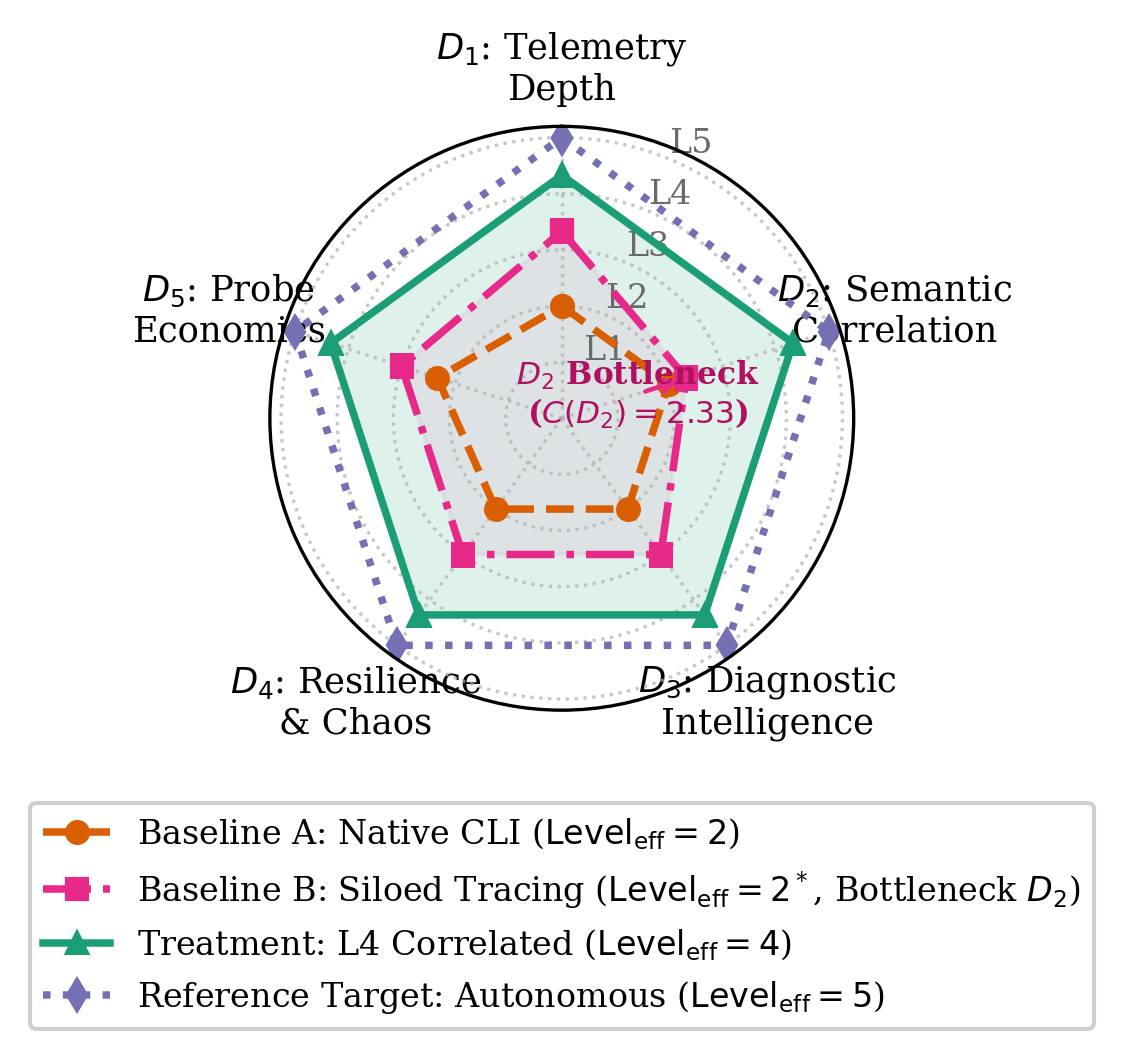
\includegraphics[width=\columnwidth]{figures/fig_omm_radar_profiles.png}
    \caption{Five-Dimensional CN-OMM Capability Profiles across Evaluated Kubernetes Regimes, Illustrating the $D_2$ Semantic Correlation Stage-Gate Bottleneck in Siloed Level 3 Tracing vs.\ Balanced Level 4 Multimodal Fusion.}
    \label{fig:omm_radar_profiles}
\end{figure}

\begin{figure*}[!t]
    \centering
    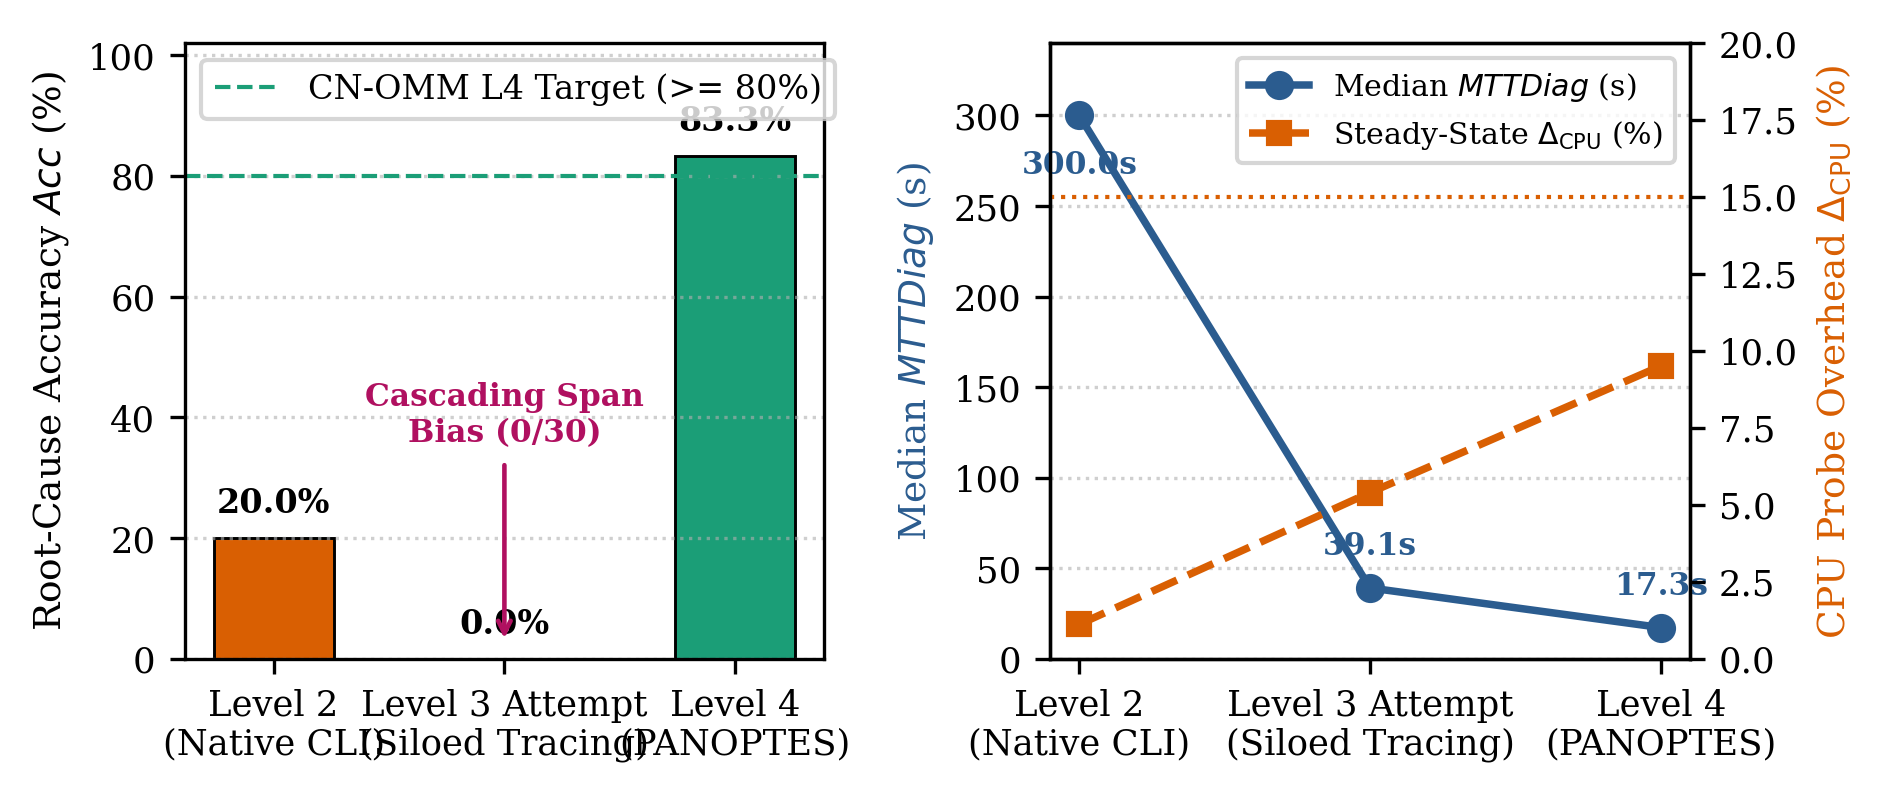
\includegraphics[width=0.92\textwidth]{figures/fig_omm_pareto_frontier.png}
    \caption{Empirical Performance Trajectory across CN-OMM Maturity Stages: Root-Cause Diagnostic Accuracy ($Acc$), Median Diagnostic Latency ($MTTDiag$), and Steady-State CPU Probe Effect ($\Delta_{\text{CPU}}$) over $N=30$ Paired Chaos Trials.}
    \label{fig:omm_pareto_frontier}
\end{figure*}

\subsubsection{Empirical Proof of the Monomodal Additivity Fallacy (Level 3 Bottleneck)}
A striking empirical finding in Table~\ref{tab:empirical_validation} is the performance of \textbf{Baseline B (Siloed Tracing)}. Under a traditional compensatory maturity model, Baseline B scores an arithmetic mean of $\bar{C} = 2.92 \approx \text{Level 3}$ because it deploys distributed tracing SDKs ($D_1 = 3.3$) and reduces symptom detection latency to a median of $39.15\,\text{s}$. However, its root-cause localization accuracy collapses to \textbf{$0.00\%$ ($0/30$ correct diagnoses)}---performing worse than basic Level 2 CLI inspection ($20.00\%, 6/30$).

In every single trial ($30/30$), ranking spans by inclusive duration $D(s_i)$ caused the monomodal trace engine to blame the upstream ingress gateway (\texttt{frontend}) rather than the true downstream fault (\texttt{paymentservice}, \texttt{cartservice}, or \texttt{checkoutservice}), confirming our mathematical formulation of \textbf{Cascading Span Bias} in Equation~(\ref{eq:inclusive_duration}). Crucially, the CN-OMM's non-compensatory Stage-Gate equation ($\text{Level}_{\text{eff}} = \min_k \lfloor C(D_k) \rfloor = 2$) accurately predicts this failure by flagging the configurational bottleneck in $D_2 = 2.3$ (absence of $T_{\text{self}}$ decomposition and cross-pillar log/metric correlation).

\subsubsection{Quantitative Breakthrough at CN-OMM Level 4 (Correlated Multimodal Fusion)}
When the cluster satisfies all five dimensional stage-gates at \textbf{Level 4 ($\text{Level}_{\text{eff}} = 4, \mathcal{I}(\mathcal{S}) = 0.833$)}, diagnostic performance exhibits a statistically decisive phase transition:
\begin{itemize}[leftmargin=*, nosep]
    \item \textbf{Root-Cause Accuracy ($Acc$):} Jumps from $20.00\%$ (Level 2) and $0.00\%$ (siloed Level 3) to \textbf{$83.33\%$ ($25/30$)} (Fisher's exact $p = 7.74 \times 10^{-7}$, odds ratio $\text{OR} = 20.0$; McNemar's paired $p = 7.83 \times 10^{-5}$). Stratified by fault type, Level 4 achieves $90\%$ accuracy on network degradation ($9/10$), $80\%$ on abrupt pod termination ($8/10$), and $80\%$ on CPU saturation ($8/10$).
    \item \textbf{Diagnostic Latency ($MTTDiag$):} Plummets by \textbf{$94.24\%$} from a median of $300.00\,\text{s}$ ($\text{IQR} = 0.0\,\text{s}$) in Level 2 to \textbf{$17.27\,\text{s}$ ($\text{IQR} = 5.91\,\text{s}$)} in Level 4 (Wilcoxon signed-rank $p = 3.06 \times 10^{-5}$, Vargha-Delaney $\hat{A}_{12} = 0.817$ [large effect], Cliff's $\delta = +0.633$).
    \item \textbf{Dimension $D_5$ (Probe Effect Governance):} Across continuous steady-state profiling, the full Level 4 multimodal pipeline imposes a marginal CPU overhead of \textbf{$\Delta_{\text{CPU}} = 9.51\% \pm 2.14\%$} (95\% CI $[8.71\%, 10.31\%]$), remaining statistically well below the $15.0\%$ stability budget (one-sample $t$-test $t = -14.05, p = 6.52 \times 10^{-9}$).
    \item \textbf{Dimension $D_4$ (Chaos Verification Overhead Invariance):} Furthermore, our $N=60$ cross-engine verification confirms that coupling Level 4 observability with resident eBPF/DaemonSet chaos injectors (Chaos Mesh) vs.\ transient Pod injectors (LitmusChaos) preserves steady-state application latency while isolating control-plane scheduling overhead ($141\,\text{ms}$ vs.\ $3{,}840\,\text{ms}$, $p = 1.73 \times 10^{-6}$), enabling continuous automated verification of $\text{QCI}_{4.2}$ in production.
\end{itemize}
